\documentclass[12pt]{article}

\usepackage[utf8]{inputenc}
\usepackage[brazil]{babel}
% \usepackage[english]{babel}

\usepackage{amsmath,amsthm,amsfonts,amssymb}
\usepackage{graphicx,enumerate}
\usepackage{hyperref}
\usepackage{float}
\usepackage{booktabs}
\usepackage[normalem]{ulem}
% \useunder{\uline}{\ul}{}
\usepackage{multirow}
\usepackage[table,xcdraw]{xcolor}
\usepackage{systeme}
\usepackage{array}
\usepackage{makecell}
\usepackage{afterpage}
\usepackage{algorithm} 
\usepackage{algpseudocode}
\usepackage{longtable}
\usepackage{adjustbox}
\usepackage{rotating}
\usepackage{quotes}
\usepackage{caption, subcaption}
\usepackage{etoolbox}

% My customization

%% Hide link boxes
\hypersetup{hidelinks}

%% Custom commands
% !TEX root = ../pmaluminum.tex


%%%%%%%%%%%%%%%%%%%
% My commands
%%%%%%%%%%%%%%%%%%%

\newcommand{\goal}[1]{[\textbf{Goal:} \blue{\emph{#1}}]}
\newcommand{\todo}[1]{[\textbf{TODO:} \cyan{\emph{#1}}]}
\newcommand{\question}[1]{[\emph{\textbf{Q:} \orange{#1}}]}
\newcommand{\todoeq}{[\green{\emph{EQ}}]}
\newcommand{\todofig}{[\green{\emph{FIG}}]}
% \newcommand{\source}[1]{[\green{\emph{src}#1}]}
\newcommand{\source}[1]{%
  \ifstrempty{#1}%
    {\green{[\emph{src}]}}%
    {\green{[\emph{#1} ]}}%
}


\newcommand{\diff}{\mathrm{d}}
\newcommand{\delScalar}[2]{\frac{\partial #1}{\partial #2}}
\newcommand{\delScalarSq}[2]{\frac{\partial^2 #1}{\partial #2^2}}
\newcommand{\delScalarTwo}[3]{\frac{\partial^2 #1}{\partial #2\partial #3}}
\newcommand{\delVector}[2]{\frac{\partial \mathbf{#1}}{\partial #2}}
\newcommand{\dScalar}[2]{\frac{\diff #1}{\diff #2}}
\newcommand{\dScalarSq}[2]{\frac{\diff^2 #1}{\diff #2^2}}
\newcommand{\dVector}[2]{\frac{\diff \mathbf{#1}}{\diff #2}}
\newcommand{\Nabla}{\boldsymbol{\nabla}}
\newcommand{\dr}[1]{\ \diff_{\mathrm{r}}\left(#1\right)}
\newcommand{\dt}[1]{\ \diff_{\mathrm{t}}\left(#1\right)}
% \newcommand{\dt}[1]{\dScalar{#1}{t}}

\newcommand{\cyan}[1]{\colorbox{cyan}{#1}}
\newcommand{\blue}[1]{\colorbox{blue}{#1}}
\newcommand{\red}[1]{\colorbox{red}{#1}}
\newcommand{\green}[1]{\colorbox{green}{#1}}
\newcommand{\yellow}[1]{\colorbox{yellow}{#1}}
\newcommand{\orange}[1]{\colorbox{orange}{#1}}

\newcommand{\Sh}{\mathrm{Sh}}
\newcommand{\Nu}{\mathrm{Nu}}
\newcommand{\Le}{\mathrm{Le}}
\newcommand{\Sc}{\mathrm{Sc}}
\newcommand{\Bi}{\mathrm{Bi}}
\newcommand{\Reynolds}{\mathrm{Re}}
\newcommand{\Prandtl}{\mathrm{Pr}}

\newcommand{\qAl}{\mathrm{Al}}
\newcommand{\qO}{\mathrm{O}}
\newcommand{\qH}{\mathrm{H}}
\newcommand{\qC}{\mathrm{C}}
\newcommand{\qN}{\mathrm{N}}
\newcommand{\qCO}{\mathrm{CO}}
\newcommand{\qAlAlOOO}{\qAl_2 \qO_3}
% \newcommand{\qH2O}{\H_2\O}
% \newcommand{\H}{\H_2}

\newcommand{\mrm}[1]{\mathrm{#1}}

\newcommand{\ejected}{\mrm{ejected}}
\newcommand{\const}{\mrm{const}}
\newcommand{\cond}{\mrm{cond}}
\newcommand{\conv}{\mrm{conv}}
\newcommand{\comb}{\mrm{comb}}
\newcommand{\melt}{\mrm{melt}}
\newcommand{\evap}{\mrm{evap}}
\newcommand{\boil}{\mrm{boil}}
\newcommand{\film}{\mrm{film}}
\newcommand{\rad}{\mrm{rad}}
\newcommand{\dep}{\mrm{dep}}
\newcommand{\net}{\mrm{net}}
\newcommand{\env}{\mrm{env}}
\newcommand{\flm}{\mrm{flm}}
\newcommand{\HSR}{\mrm{HSR}}
\newcommand{\HGR}{\mrm{HGR}}
\newcommand{\st}{\mrm{st}}

\newcommand{\qntdd}[2]{\ensuremath{#1 \, \mathrm{#2}}}

\renewcommand{\eqref}[1]{(\ref{#1})}

\newcommand{\from}[1]{
    \\
    \vspace{0.2cm} 
    {\small 
    \textbf{From}: \citeonline{#1}.
    }}

\newcommand{\fromme}{
    \\
    \vspace{0.2cm} 
    {\small 
    \textbf{From}: present author.
    }}

%% Line spacing
\usepackage{geometry}
\geometry{a4paper,portrait,hmargin={2cm,2cm},vmargin={2cm,2.5cm}}
\renewcommand{\baselinestretch}{1.5}
\usepackage{setspace}

%% Fonstize set at line 1

%% Bibliography style bibtex (with citeonline)
    \usepackage{cite}
    %%% https://www.overleaf.com/learn/latex/Bibtex_bibliography_styles#Table_of_stylename_values
%% Bibliography style with natbib (with citeauthor)
    % \usepackage{natbib}
    %%% https://www.overleaf.com/learn/latex/Natbib_bibliography_styles
%% Bibliography style ABNTEX2 with citeonline
    % \usepackage[alf]{abntex2cite} 
    %%% See https://mirrors.ibiblio.org/CTAN/macros/latex/contrib/abntex2/doc/abntex2cite-alf.pdf

%% Include References in toc
\usepackage[nottoc]{tocbibind}

%% Dummy text
\usepackage{lipsum}

%% Line numbers
\usepackage{lineno}

% % Blank page
% \usepackage{afterpage}

% \title{\textbf{Multi-Scale Investigations For Reacting Multi-Phase Dispersed Spray Flows}}
\title{\textbf{Investigação Numérica dos Efeitos de Chamas Envelopadas em Chamas Turbulentas Diluídas de Sprays Líquidos Multicomponentes}}
\author{João Vinícius Hennings de Lara}
\date{Junho 2025}





\begin{document}

\pagenumbering{roman}

% \maketitle
% \begin{titlepage}
    \centering
    {\bfseries
    ESCOLA POLITÉCNICA DA UNIVERSIDADE DE SÃO PAULO \par
    PROGRAMA DE PÓS-GRADUAÇÃO EM ENGENHARIA MECÂNICA
    \par}

    \vspace*{5cm}
    
    {\Large\bfseries\setstretch{1}
        INVESTIGAÇÃO NUMÉRICA DOS EFEITOS DE CHAMAS ENVELOPADAS EM CHAMAS TURBULENTAS DE SPRAYS LÍQUIDOS MULTICOMPONENTES 
    \par}
    
    \vspace{3cm}
    
    \hrule
    
    {\vspace{1cm}\large \bfseries
        PLANO DE TRABALHO DE DOUTORADO DIRETO
    \vspace{1cm}}
    
    \hrule
    
    \vspace{3cm}

    {\bfseries
         M.SC. JOÃO VINÍCIUS HENNINGS DE LARA
    \par}
    \vspace{1.5cm}

    {\bfseries
     ORIENTADOR:\\ PROF. DR.-ING. FERNANDO LUIZ SACOMANO FILHO
     \par}
    \vfill

    {\bfseries
        JUNHO DE 2025
    \par}
\end{titlepage}
% \begin{titlepage}
    \centering
    \large
    {
    Escola Politécnica Da Universidade De São Paulo \par
    Programa De Pós-Graduação Em Engenharia Mecânica
    \par}

    \vspace*{5cm}
    
    {\bfseries\Large
    Investigação Numérica dos Efeitos de Chamas Envelopadas em Chamas Turbulentas de Sprays Líquidos Multicomponente\par}
    
    \vspace{2cm}

    \hrule
    \vspace{0.4cm}
    {\setstretch{1}
    Projeto de Pesquisa para Doutorado Direto\par
    Submetido à Fundação de Amparo à Pesquisa do Estado de São Paulo (FAPESP)
    }    
    \vspace{0.4cm}
    \hrule
    
    \vspace{3cm}
    {
    M.Sc. João Vinícius Hennings de Lara\par
    }
    
    \vspace{1.5cm}
    {
    Orientador:\\ Prof. Dr.-Ing. Fernando Luiz Sacomano Filho
    }
    
    \vfill
    São Paulo, Junho de 2025

\end{titlepage}

\begin{titlepage}
    \centering
    \large
    {
    Escola Politécnica da Universidade de São Paulo \par
    Programa de Pós-Graduação em Engenharia Mecânica
    \par}

    \vspace*{3.5cm}
    
    {\bfseries\Large % # TODO Atualizar SAGE
    Investigação Numérica da Queima Individual de Gotas em Chamas Turbulentas de Sprays Multicomponentes\par}
    
    \vspace{1cm}

    {\Large % # TODO Atualizar SAGE
    Numerical Investigation of Single Droplet Combustion in Turbulent Multicomponent Spray Flames\par}

    \vspace{2.5cm}

    \hrule
    \vspace{0.4cm}
    {\setstretch{1}
    Projeto de Pesquisa para Doutorado Direto\par
    Submetido ao Programa de Pós-Graduação em Engenharia Mecânica (PPGEM)
    }    
    \vspace{0.4cm}
    \hrule
    
    \vspace{3.5cm}
    {
    M.Sc. João Vinícius Hennings de Lara\par
    }
    
    \vspace{1.0cm}
    \begin{flushleft}
        Orientador:\\
    \end{flushleft}
    \vspace{-.3cm}
    {
    Prof. Dr.-Ing. Fernando Luiz Sacomano Filho
    }
    
    \vfill
    São Paulo, Junho de 2025

\end{titlepage}

% \begin{titlepage}
    \centering
    \large
    {
    Escola Politécnica da Universidade de São Paulo \par
    Programa de Pós-Graduação em Engenharia Mecânica
    \par}

    \vspace*{6cm}
    
    {\bfseries\Large % # TODO Atualizar SAGE
    Investigação Numérica da Queima Individual de Gotas em Chamas Turbulentas de Sprays Multicomponentes\par}
    % Numerical Investigation of Single Droplet Combustion in Turbulent Multicomponent Spray Flames

    \vspace{3cm}

    \hrule
    \vspace{0.4cm}
    {\setstretch{1}
    Projeto de Pesquisa para Doutorado Direto\par
    Submetido à Fundação de Amparo à Pesquisa do Estado de São Paulo (FAPESP)
    }    
    \vspace{0.4cm}
    \hrule
    
    \vspace{3cm}
    {
    M.Sc. João Vinícius Hennings de Lara\par
    }
    
    \vspace{1.5cm}
    {
    Orientador:\\ Prof. Dr.-Ing. Fernando Luiz Sacomano Filho
    }
    
    \vfill
    São Paulo, Junho de 2025

\end{titlepage}

% \begin{titlepage}
    \centering
    \large
    {
    Escola Politécnica da Universidade de São Paulo \par
    Programa de Pós-Graduação em Engenharia Mecânica
    \par}

    \vspace*{6cm}
    
    {\bfseries\Large % # TODO Atualizar SAGE
    Numerical Investigation of Single Droplet Combustion in Turbulent Multicomponent Spray Flames\par}

    \vspace{3cm}

    \hrule
    \vspace{0.4cm}
    {\setstretch{1}
    Research Project for Doutorado Direto\par
    Sumbitted to Fundação de Amparo à Pesquisa do Estado de São Paulo (FAPESP)
    }    
    \vspace{0.4cm}
    \hrule
    
    \vspace{3cm}
    {
    M.Sc. João Vinícius Hennings de Lara\par
    }
    
    \vspace{1.5cm}
    {
    Supervisor:\\ Prof. Dr.-Ing. Fernando Luiz Sacomano Filho
    }
    
    \vfill
    São Paulo, June 2025

\end{titlepage}

% \begin{titlepage}
    \centering
    \large\bfseries
    ESCOLA POLITÉCNICA DA UNIVERSIDADE DE SÃO PAULO
    PROGRAMA DE PÓS-GRADUAÇÃO EM ENGENHARIA MECÂNICA

    \vspace*{4cm}

    % Nome do autor
    JOÃO VINÍCIUS HENNINGS DE LARA

    \vspace{3cm}

    INVESTIGAÇÃO NUMÉRICA DOS EFEITOS DE CHAMAS ENVELOPADAS EM CHAMAS TURBULENTAS DE SPRAYS LÍQUIDOS MULTICOMPONENTE

    \vspace{4cm}

    PLANO DE TRABALHO DE DOUTORADO DIRETO

    \vfill

    SÃO PAULO\\
    2024
\end{titlepage}


% !TeX root = ..\Proposta.tex

\vspace{2cm}

{ \Large \textbf{Resumo}}

\vspace{0.8cm}

{
\setstretch{1}

\noindent % Se mudar aqui, lembrar de mudar no SAGE também!
A combustão turbulenta de spray é um processo essencial em diversas tecnologias. 
Sua modelagem e simulação fazem parte do esforço atual de transição energética e descarbonização.
Simulações de combustão de sprays diluídos, baseadas na dinâmica dos fluidos computacional, geralmente utilizam modelos de evaporação e condensação para as gotas.
Estes descrevem uma frente de chama externa às gotas, estabilizada pela mistura vapor-oxidante formada pela evaporação do combustível.
No entanto, chamas estabilizadas ao redor de gotas individuais também são observadas em experimentos e simulações.
Também denominadas combustão de gotas isoladas, essas chamas estão relacionadas ao processo de ignição de sprays e à formação de fuligem.
No entanto, a sua modelagem é raramente incluída em simulações computacionais.
Este trabalho visa desenvolver modelos de combustão de gota isolada (MCGI) e incluí-los em simulações de combustão turbulenta multidimensional para investigar a sua influência na combustão de sprays.
Esse desenvolvimento inclui a elaboração de modelos de evaporação e condensação (MEC).
Ambos devem ser capazes de representar efeitos de combustíveis comerciais, que são multicomponentes (como a gasolina) e/ou hidrofílicos (como o etanol e o metanol). 
Para tanto, devem ser considerados também fenômenos de transporte no interior da gota e termodinâmica de mistura não ideal.
Dessa forma, um segundo objetivo deste trabalho é avaliar os impactos do aumento de capacidade descritiva de modelos de transferência de calor e massa (MEC e MCGI) na combustão de sprays multicomponentes.
A co-utilização de MEC e MCGI em uma simulação, como proposto, deve ser acompanhada por um mecanismo de seleção de modos de combustão, a ser desenvolvido, que escolherá qual modelo utilizar para cada gota.
Esse trabalho contribuirá para o aperfeiçoamento da capacidade preditiva de simulações de chama turbulenta multidimensional de sprays multicomponentes.
% Os modelos desenvolvidos serão testados isoladamente e em uma chama laminar de névoa de spray, quiescente e monodispersa, antes de serem utilizados em simulações de chamas multidimensionais turbulentas. 
% #DONE Motivação
% #DONE Objetivo
% Primeiramente, o novo modelo será testado de forma isolada, para garantir o correto funcionamento e implementação. 
% Em seguida, será testado no cenário simplificado de uma chama laminar de névoa quiescente de spray líquido monodisperso.
% Por fim, após aprofundamento em interação chama-turbulência, o modelo será utilizado em simulações multidimensionais turbulentas.
% # DONE Resultado e contribuição para comunidade científica
% Sugestão Sacomano:
%  O desenvolvimento desse trabalho deve contribuir para o aperfeiçoamento da capacidade preditiva de ... por programas baseados na dinâmica dos fluidos computacional (CFD).

}
\vspace{1cm}

{ \Large \textbf{Abstract}}

\vspace{0.8cm}

{
\setstretch{1}

% #TODO Update translation
\noindent % Se mudar aqui, lembrar de mudar no SAGE também!
The modeling of turbulent diluted spray flame is usually modelled using evaporation and condensation models, which produces an external flame sheet.
Nonetheless, enveloped flames around isolated droplets have already been seen in experiments and simulations of turbulent liquid spray flames.
Also named single or isolated droplet combustion, these flames have already been related to spray ignition processes and formation of soot.
Reviewing the literature, it was clear that the modeling of enveloped flames should be included in simulations of turbulent diluted liquid spray flames. 
The development of such models ought to represent real fuels which are mixtures of diferent chemical species, like kerosene, and/or hydrophilic, like ethanol.  
Therefore they must be able to represent multicomponent mixtures, to consider transport phenomena inside the droplet and to consider non-ideal mixture thermodynamics.
Developing single droplet combustion models (MCGI) will encompass the developement of evaporation and condensation models (MEC) with the same capabilities, thus ensuring a gradual model development process, which will be based on pre-existing models in the literature.
The simultaneous use of MEC and MCGi in a simulation must include a switch, also to be developed, that will chose which model to apply to each droplet.
The new model will first be tested independently, to ensure its correct working and implementation.
Then, it will be tested in the simplified cenario of a laminar flame in a quiescent monodisperse droplet mist.
Lastly, after investigating flame-turbulence interaction, the model will be used in multidimensionais turbulent spray flame simulations.

}

\newpage
\tableofcontents
\newpage

\newcounter{savecounter} 
\setcounter{savecounter}{\value{page}} 
\pagenumbering{arabic} 

\section{Introdução} \label{sec:intro}

A crescente demanda por transição energética e pela descarbonização da economia impulsiona a busca por alternativas aos combustíveis fósseis nos setores de energia, transporte, indústria. 
Alguns setores, como o de transporte urbano de veículos leves, têm apresentado avanço significativo na utilização de energias renováveis e na eletrificação \cite{MasriA2021}. 
Porém, combustíveis fósseis são extremamente difíceis de substituir em outros setores, especialmente quando se trata de combustíveis líquidos.
Estes possuem maior energia específica e densidade energética quando comparados com outras fontes de energia, como combustíveis gasosos ou baterias elétricas \cite{Bergthorson2017,Julien2017}.
São assim adequados para aplicações de transporte, como no setor automotivo de cargas pesadas, naval e aeronáutico \cite{MasriA2021}.
Combustíveis líquidos são importantes também para algumas indústrias como aço e cimento, para algumas termoelétricas e até para máquinas portáteis movidas a motor de combustão interna (MCI).
Ademais, uma análise histórica indica que a transição para fontes renováveis se dará ao longo de décadas \cite{MasriA2021}.

% Nota-se que processos de combustão continuarão relevantes nas próximas décadas.
Todas as aplicações mencionadas anteriormente baseiam-se na combustão turbulenta de sprays líquidos.
Assim, é necessário buscar soluções que conciliem essa tecnologia com os esforços de transição energética e descarbonização da economia.
A comunidade científica e a indústria têm dado ênfase nas seguintes demandas: \textbf{(i)} desenvolver tecnologias para o uso de novos combustíveis (como  etanol, metanol, hidrogênio e amônia) \cite{MasriA2021,FAPESP_etanol_1,VerhelstS2019,TeohY2023,ElbazA2022}; \textbf{(ii)} desenvolver novas rotas de produção para combustíveis já utilizados (resultando, por exemplo, nos chamados SAF, biocombustíveis e eletro-combustíveis \cite{MasriA2021,BenJames-SAF,BergthorsonJ2015,WestbrookC2019,PalysM2022}); \textbf{(iii)} melhorar a eficiência dos \emph{"prime-movers"} a combustão e reduzir a formação de poluentes \cite{MasriA2021}.

Independente da origem do combustível, o processo de combustão deve ser bem compreendido para que \emph{"prime-movers"} e queimadores eficientes e com baixa emissão de poluentes sejam desenvolvidos.
Para tanto é necessário pesquisa em combustão, que pode ser estruturada em trabalhos experimentais e trabalhos de modelagem.
A modelagem da combustão turbulenta de sprays, foco dessa proposta, deve ser capaz de contemplar diferentes combustíveis líquidos, incluindo combustíveis oriundos das demandas (i) e (ii).
Deve também representar os diferentes fenômenos envolvidos nesse processo, como ignição e formação de poluentes, para atender a demanda (iii).
No âmbito da combustão turbulenta de sprays, é de extrema importância o modelo de transferência de calor e massa da gota (líquida) para a fase gasosa (HMT -\emph{Heat and Mass Transfer}).
Modelos HMT regem, dentre outros aspectos, a taxa de vaporização do combustível das gotas do spray.
É conhecido que essa modelagem tem enorme influência na chama, afetando sua estrutura, distribuição de temperatura, geometria e formação de poluentes \cite{JennyB2012}.


Nesse sentido, revisando a literatura mais recente, nota-se a necessidade de maior desenvolvimento de \textbf{modelos de evaporação e condensação} (MEC) computacionalmente eficientes capazes de representar corretamente diferentes combustíveis.
Por exemplo, modelos monocomponentes com equilíbrio termodinâmico, embora computacionalmente eficientes, não são capazes de representar todos os fenômenos associados à combustão de combustíveis hidrofílicos, como o etanol \cite{SacomanoF2024CF}, combustível de importância estratégica para o Brasil \cite{etanol-BNDES} e também para outros países, como a Índia \cite{etanol-India}.
Para descrever combustíveis comerciais como o etanol é necessário modelar a gota com abordagem de substância \textbf{multicomponente}, considerando \textbf{termodinâmica de mistura não-ideal} e os efeitos de transferência de calor e massa no \textbf{interior da gota} \cite{SacomanoF2024CF}.
% Em especial, nota-se uma demanda pela aplicação de modelos que tenham a capacidade de descrever diversos fenômenos subjacentes à combustão de sprays multicomponentes e computacionalmente robustos para serem utilizados na simulação de chama turbulenta de spray.  
% Em especial, nota-se uma demanda pela aplicação de modelos detalhados, desenvolvidos e testados em cenários simplificados, como na escala de uma única gota ou em simulações laminares ou unidimensionais, em simulações multidimensionais de combustão turbulenta.

Em MECs, a evaporação da gota fornece vapor de combustível que alimenta a chama.
Nessa abordagem, a chama não é estabilizada por uma gota em específica, mas se estabilizada por fenômenos específicos ao escoamento gasoso \cite{ChiuH1982,Law2006}.
Esse modo de combustão de spray é chamado \textbf{combustão com frente de chama externa}, ou simplesmente \textbf{combustão externa}.
Em contraste, é possível que as gotas entrem em combustão individualmente, com a evaporação de combustível alimentando uma frente de chama próxima e envolvente a cada gota, a uma distância na mesma ordem de grandeza que o diâmetro da gota \cite{ChiuH1977}.
Isso é chamado \textbf{combustão de gota isolada}.

Experimentos indicam que a combustão de gota isolada ocorre tanto durante a ignição	de sprays \cite{AggarwalS2014} quanto em sprays já desenvolvidos \cite{ChenG1996CF,GounderJ2009PhD,SinghG2020}.
Simulações DNS (\emph{Direct Numerical Simulation}) e LES (\emph{Large Eddy Simulation}) também indicam a ocorrência de combustão de gota isolada nessas duas etapas da combustão turbulenta de sprays líquidos, como em \cite{BorghesiG2013CF} e \cite{PaulhiacD2020,BojkoDesJardin2017CF}, respectivamente.
A combustão de gota isolada também ocorre na combustão de alguns pós metálicos como o alumínio \cite{Bergthorson2015,Julien2017,Baumann2020}, segundo várias evidências experimentais \cite{Braconnier2020Pre,Braconnier2022,Bucher1999,Halter2023}.
A Figura \ref{fig:sdc-exp} mostra evidências da combustão de gota isolada em sprays turbulentos de etanol (Figuras \ref{fig:GounderJ2009-7.17} e \ref{fig:SinghG2020-10}) e na combustão de uma partícula alumínio (Figura \ref{fig:Braconnier202PhD-5.20}). %\todo{explicar figuras ...}

Além disso, alguns trabalhos apontam para a combustão de gota isolada em sprays líquidos como uma fonte de emissão de fuligem \cite[e as referências 3-13 ali citadas]{FachiniF2005}, de forma que a modelagem desse fenômeno contribui com os esforços de limitar as emissões de material particulado.

\begin{figure}[H]
    \centering
    \caption{Observações experimentais de combustão de gota isolada em chamas de etanol na Fig. \ref{fig:GounderJ2009-7.17} e \ref{fig:SinghG2020-10}, indicadas por setas, e ao redor de uma partícula de pó de alumínio na Fig. \ref{fig:Braconnier202PhD-5.20}. 
    Siglas: LIF -- \emph{Laser Induced Fluorescence}; HR -- \emph{Heat Release}.
    Adaptadas de \cite{GounderJ2009PhD,SinghG2020,Braconnier2020Pre}.
    }
    \begin{subfigure}[t]{0.32\textwidth}
        \centering
        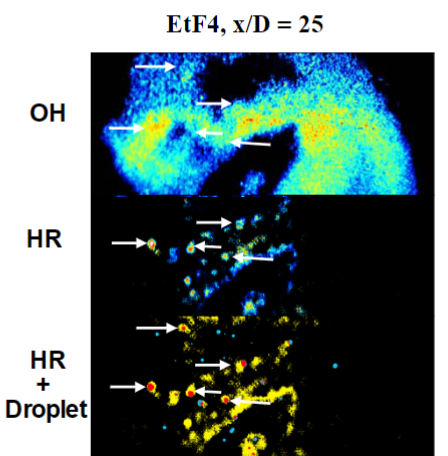
\includegraphics[width=0.99\textwidth]{30_images/GounderJ2009-7.17-1.png}
        \caption{LIF de OH, HR e HR sobreposto com posição das gotas em uma chama de etanol no queimador \emph{Sydney Dilute Spray Burner}, 25 diâmetros do injetor a jusante. Adaptado de \cite[Fig. 7.13]{GounderJ2009PhD}.}
        \label{fig:GounderJ2009-7.17}
    \end{subfigure}
    \begin{subfigure}[t]{0.48\textwidth}
        \centering
        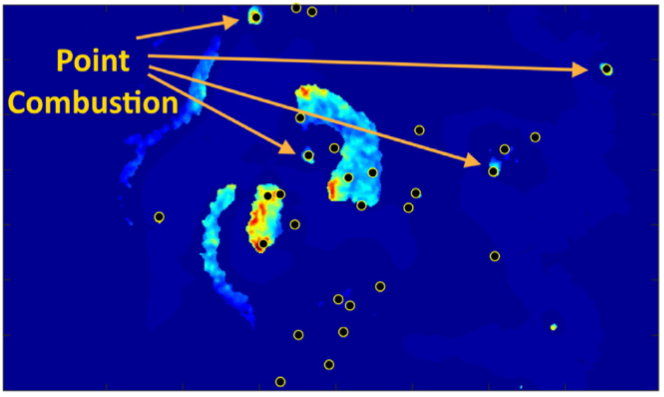
\includegraphics[width=0.99\textwidth]{30_images/SinghG2020-10.png}
        \vfill
        \caption{HR sobreposto com posição das gotas em uma chama de etanol no queimador \emph{Sydney Piloted Needle Spray Burner}, 20 diâmetros do injetor a jusante. Adaptado de \cite[Fig. 10]{SinghG2020}.}
        \label{fig:SinghG2020-10}
    \end{subfigure}
    \vspace{0.5cm}
    \begin{subfigure}[b]{0.8\textwidth}
        \centering
        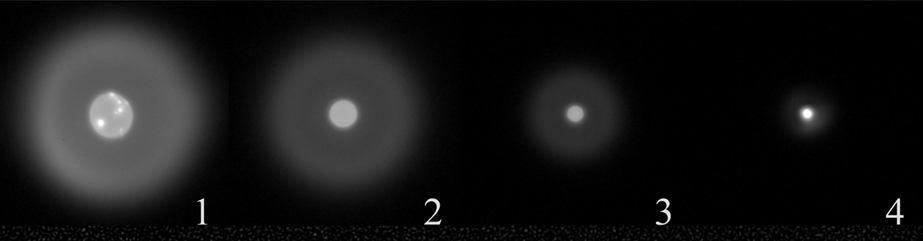
\includegraphics[width=0.99\textwidth]{30_images/Braconnier202PhD-5.20.png}
        \caption{Fotografias de combustão de uma partícula de alumínio de $\qntdd{50}{\mu m}$ de diâmetro em atmosfera 80\% Argônio/ 20\% oxigênio. Adaptado de \cite[Fig. 5.21]{Braconnier2022}.}
        \label{fig:Braconnier202PhD-5.20}
    \end{subfigure}
    \label{fig:sdc-exp}
\end{figure}
\vspace{-24pt}

Diante dos aspectos expostos, nota-se que modelar a combustão de gota isolada é de grande importância para a descrição da ignição de sprays de combustíveis líquidos, da emissão de poluentes (em particular de fuligem) e também para a descrição da combustão de alguns combustíveis metálicos. 
Revisando a literatura, constatou-se a necessidade de desenvolver \textbf{modelos de combustão de gota isolada} (MCGI) capazes de representar corretamente diferentes combustíveis, incluindo as mesmas capacidades encontradas no chamado estado-da-arte para os MECs.
Notou-se também que não é claro na literatura quando a combustão de gota isolada ocorre \cite[p. 8]{JennyB2012} -- apesar de existirem diferentes modelos em cenários simplificados, a serem discutidos -- nem a influência de modelar a combustão de gota isolada (representada por MCGIs) junto com a combustão externa (representada por MECs) na combustão turbulenta multidimensional.


\subsection{Objetivos} \label{sec:objetivos}

Tendo em vista os aspectos levantados anteriormente, este trabalho tem como objetivo avaliar os impactos do aumento de capacidade descritiva de modelos HMT em sprays multicomponentes e avaliar a influência da combustão de gota isolada na combustão de spray.
Para isso, esse trabalho propõe o desenvolvimento de estratégias para a simulação da transferência de calor e massa em gotas em dois cenários: (\textbf{A.}) combustão externa; (\textbf{B}.) combustão de gota isolada.
Esses cenários correspondem aos seguintes modelos HMT:
\begin{enumerate}
    \item[\textbf{A.}] Modelo de Evaporação e Condensação (MEC); e 
    \item[\textbf{B.}] Modelo de Combustão de Gota Isolada (MCDI).
\end{enumerate}
Esses modelos devem considerar os seguintes aspectos: 
\begin{enumerate}
    \item[\textbf{1.}] Descrição multicomponente da gota; 
    \item[\textbf{2.}] Gota com termodinâmica de mistura não-ideal; 
    \item[\textbf{3.}] Consideração dos efeitos de transferência	de calor e massa no interior da gota. 
\end{enumerate}
O objetivo é desenvolver aplicar a estratégia desenvolvida em simulações turbulentas reativas multidimensionais, com ambos modelos, {A} e {B} e com a funcionalidade:
\begin{enumerate}
    \item[\textbf{4.}] Determinação de quando ocorre a combustão de gota isolada;
\end{enumerate}
ou seja, de determinar se a gota se encontra no cenário {A} ou {B} e escolher o modelo apropriado para a correta representação dos fenômenos envolvidos.
Visando a aplicação em simulações CFD (\emph{Computational Fluid Dynamics}) turbulentas, reativas e multidimensionais, as estratégias a serem desenvolvidas devem ser robustas e computacionalmente eficientes.

Simulações CFD com um modelo HMT que utilize as estratégias a serem desenvolvidas, incluindo as funcionalidades {1}, {2}, {3} e {4}, terão maior complexidade teórica em comparação aos modelos utilizados pela literatura. 
Isso permitirá ao autor dessa proposta investigar o efeito de considerar a combustão de gota isolada, e dos aspectos {1}, {2} e {3}, na estrutura da chama.
A investigação da estrutura da chama inclui a investigação de aspectos como distribuição de temperatura e concentrações de espécies, o que é essencial para a determinação da ignição, da eficiência de combustão e das emissões de poluentes.
% A relação da estratégia a ser desenvolvida \yellow{com a emissão de poluentes e com a ignição de sprays também será investigada.}    % Introdução Justificativa e síntese da bibliografia fundamental
% !TEX root = ../Proposta.tex


\section{Fundamentação Teórica}


\subsection{Combustão Turbulenta de Sprays} \label{sec:teoria}

%  devido às instabilidades hidrodinâmicas de Kevin-Helmholz e Rayleigh-Taylor, formando gotas que se dispersam, eventualmente se deformam e se rompem quando as forças aerodinâmicas superam as tensões superficiais da gota, formando novas gotas \cite{JennyB2012}.
% Isso forma a \textbf{região densa} do spray, onde ocorrem também outros fenômenos como colisões, coalescência e interferência por esteira aerodinâmica, por turbulência ou por alteração da concentração de vapor de combustível devido à evaporação.
A combustão turbulenta de sprays é caracterizada pela competição de vários fenômenos físicos e químicos, fortemente acoplados e em diferentes escalas de tempo e comprimento. 
Na formação de um spray turbulento, um jato de combustível líquido se quebra em gotas menores nos processos de atomização primária e secundária \cite{JennyB2012}.
A região inicial do spray, chamada de \textbf{densa}, é caracterizada por fenômenos de interação entre gotas, como colisões, coalescência e interferência por esteira aerodinâmica.
A medida que as gotas se tornam menores e mais dispersas, elas deixam de interferir umas nas outras e o spray é chamado de \textbf{disperso} ou \textbf{diluído}. 
Desde a sua formação, as gotas de combustível evaporam, fornecendo vapor combustível para a chama, que por sua vez influencia e é influenciada pelas próprias gotas e pela turbulência local.
Revisões detalhadas e com mais referências para processos e interações subjacentes à combustão turbulenta de sprays podem ser encontradas em \cite{JennyB2012, MasriA2016, SanchezA2015, ZhouL2021,JiangX2010}.

O foco deste trabalho é na modelagem de processos associados à mudança de fase da gota (escala micro), que será utilizada em simulações CFD turbulentas multidimensionais, na escala do spray e da chama (escala macro), considerando apenas a região diluída de sprays de combustível líquido.
Simulações CFD  de chamas turbulentas de spray requerem, dentre outras, a modelagem da fase contínua, gasosa, da combustão turbulenta e da fase dispersa, as gotas.
A modelagem da fase gasosa é discutida na Seção \ref{sec:gas}, seguida pela modelagem da combustão turbulenta de sprays na Seção \ref{sec:comb-sprays}. 
Por fim, a modelagem da fase discreta é apresentada na Seção \ref{sec:gotas}.
Os modelos associados à gota, escala micro, são discutidos nas seções seguintes: MECs na Seção	\ref{sec:MEC} e MCGIs na Seção \ref{sec:MCGI}.


\subsubsection{Modelagem da Fase Contínua} \label{sec:gas}

Neste trabalho, será empregada a abordagem Euler-Lagrange, na qual a fase gasosa é tratada como contínua (descrição euleriana) e as gotas líquidas são representadas como partículas pontuais (descrição lagrangiana), cuja trajetória e evolução são acompanhadas ao longo da simulação. 
As equações de transporte da fase contínua — conservação de espécie química, quantidade de movimento e energia — são discretizadas no tempo e no espaço, geralmente seguindo o Método dos Volumes Finitos  em aplicações CFD \cite{Anderson2009}.
A consideração das gotas como partículas pontuais faz-se necessária devido ao grande número de gotas no spray e à grande diferença de escalas de comprimento entre as gotas e o spray.
Nessa técnica, conhecida como \emph{Particle Source In Cell} (PSIC), a interação entre as gotas e o escoamento é representada por termos fonte nas células do domínio computacional, o que permite contabilizar os efeitos acumulados das partículas sobre a fase contínua de maneira robusta e eficiente para simulações de chama turbulenta multidimensionais.

A modelagem da fase gasosa em simulações CFD turbulentas requer um tratamento para descrever a turbulência. 
Nesse sentido, as simulações das grandes escalas (método LES) tem se mostrado bastante eficazes para a descrição da combustão turbulenta de sprays, especialmente devido a capacidade de simular fenômenos intrinsicamente transitórios como turbulência e processos envolvendo sprays \cite{SacomanoF2020CF}.
A simulação de chamas turbulentas de spray com LES, junto com o método de interação chama-turbulência ATF (\emph{Artificially Thickened Flame}), apresentado na Seção \ref{sec:comb-sprays}, vem sendo desenvolvida pelo presente grupo de pesquisa \cite{SacomanoF2017PhD,SacomanoF2017CF,SacomanoF2018CTM,SacomanoF2019Fluids,SacomanoF2020CF}.

Nessa abordagem, as variáveis transportadas são espacialmente filtradas de acordo com $\psi = \widetilde\psi + \psi^"$ usando um filtro de comprimento $\Delta_{malha}$. $\psi^"$ são as flutuações sub-escala (SGS - \emph{sub-grid scale}) e $\widetilde\psi$ representa a quantidade filtrada espacialmente, ponderada pela massa específica, $\widetilde\psi = \overline{\rho\psi}/\overline\rho$.
Utilizando uma formulação de densidade variável para baixos números de Mach, as equações de transporte de massa e de quantidade de movimento são
\begin{equation}
    \frac{\partial \overline \rho}{\partial t} + 
    \frac{\partial \overline \rho \widetilde u_j}{\partial x_j} = 
    \overline S_m,
\end{equation}
\begin{equation}
    \frac{\partial \overline\rho \widetilde u_i}{\partial t} + 
    \frac{\partial \overline\rho \widetilde u_i \widetilde u_j}{\partial x_j} =
    \frac{\partial }{\partial x_j} \left(
        2\overline\mu \widetilde S_{ij} -
        \frac{2}{3}\overline\mu \frac{\partial \widetilde u_k}{\partial x_k} \delta_{ij} -
        \overline\rho \tau_{ij}^{\text{sgs}}
    \right) -
    \frac{\partial \overline p}{\partial x_i} +
    \overline p g_i + 
    \overline S_{u,i}.
\end{equation}
Na equação de transporte de massa da mistura, $\rho$ é a massa específica da mistura, $t$ é o tempo, $u_j$ os componentes da velocidade na direção $j$ ($j=1,2,3$).
Na equação de transporte de quantidade de movimento, $\mu$ é a viscosidade dinâmica, $S_{ij}$ é o tensor da taxa de deformação, $\delta_{i,j}$ é o delta de Kronecker, $p$ é a pressão e $g_i$ é o componente da aceleração da gravidade na direção	$i$ ($i=1,2,3$). 
Os termos de acoplamento entre fases devido à presença da fase dispersa, $S_m$ e $S_{u,i}$,  são termos fontes de massa e de quantidade de movimento, respectivamente.
É através desses termos que os efeitos das gotas são considerados na fase gasosa.
$\tau_{ij}^{sgs}$ é o tensor das tensões originados pelos termos sub-malha.
Nos trabalhos do grupo de pesquisa, os termos de acoplamento entre fase seguem a implementação de Chrigui\etal{} \cite{ChriguiM2012} e o tensor SGS é fechado utilizando o modelo sigma \cite{NicoudF2011}.
% de Smagorinski \cite{Pope2000} com o procedimento dinâmico de Germano\etal \cite{Germano1991}.
% #DONE corrigir aqui. Ver correção em papel.

\subsubsection{Modelagem da Combustão Turbulenta de Sprays} \label{sec:comb-sprays}

% No contexto de combustão externa, com o uso de MECs, entende-se que a chama formada é uma chama pré-misturada, devido ao vapor de combustível evaporado pelas gotas se misturar com o oxidante do ambiente \cite{PoinsotVeynante2005}.
% No contexto de combustão externa, com o uso de MECs, em certas condições, a chama formada queima no modo de chama pré-misturada, devido ao fato de uma mistura de vapor e oxidante e oxidante chegar a chama numa proporção inflamável devido à pré-vaporização parcial \cite{PoinsotVeynante2005}.
No contexto de combustão externa, com o uso de MECs, a vaporização do combustível produz uma mistura de vapor de combustível com oxidante.
Em certas condições, essa mistura está em proporção inflamável e a chama formada queima no modo de pré-mistura \cite{PoinsotVeynante2005}.
Em simulações de combustão nas grandes escalas, a zona de reação pertence a escala sub-malha.
Ademais, a característica não linear dos termos de reação faz com que a zona de reação não seja corretamente representada pelas quantidades filtradas \cite{SacomanoF2017PhD}.
Assim, faz-se necessária a modelagem de combustão turbulenta de sprays para tratar esses problemas não resolidos.
Existem diferentes abordagens para modelar a interação chama-turbulência, que podem ser classificadas em abordagens estocásticas (baseadas em funções de distribuição de probabilidade) e  determinísticas.

% O ATF aborda a interação chama-turbulência de duas maneiras: o espessamento artificial da chama e o amarrotamento da zona de reação causado pela turbulência.
% O espessamento artificial da chama traz o efeito da interação chama-turbulência para as grandes escalas, permitindo que a resolução da chama em células típicas de LES.
% O amarrotamento da zona de reação, no contexto do ATF, é considerado por uma função de eficiência que acelera a velocidade da zona de reação.
% O ATF permite tratar a solução da zona de reação sub-malha e da interação da chama-turbulência de forma individual.
Dentre as abordagens determinísticas, se destaca o espessamento artificial da chama (ATF), que vem sendo utilizado pelo grupo de pesquisa \cite{SacomanoF2017PhD,SacomanoF2017CF,SacomanoF2020CF}.
O ATF trata tanto da solução da zona de reação sub-malha quanto da interação da chama-turbulência. 
A zona de reação sub-malha é tratada com o espessamento artificial, que permite a resolução da zona de reação em malhas de resolução típicas de LES, enquanto a interação da chama espessada com a turbulência, que resulta no amarrotamento da chama, é modelada por uma função de eficiência. 
Embora o método ATF apresente restrições teóricas para descrever os múltiplos modos de chama existentes em muitos processos de combustão de spray, ele tem importância especial para o estudo de interações interfásicas em processos de combustão de sprays. 
Ao espessar a chama e permitir a identificação da zona de reação a todo momento, as interações interfásicas podem ser claramente identificadas e a validade da abordagem PSIC é preservada.
Os efeitos do espessamento artificial e do amarrotamento de chama se manifestam na equação de transporte de um escalar $\psi$ através dos fatores de espessamento $F$ e da função de eficiência $E$.
A equação de transporte é a mesma para os escalares  $\psi=\lbrace Y_{pv}, Z, h\rbrace$, ou seja, para a variável de progresso, para a fração de mistura, e para a energia (expressa em termos da entalpia total). As duas primeiras são definidas como combinações lineares de, respectivamente, frações mássicas de elementos e de espécies químicas, ambas atendendo a condições específicas \cite{PoinsotVeynante2005,vanOijen2016PECS}.
Em uma formulação de densidade variável para baixos números de Mach, essa equação tem a forma
\begin{equation}
    \frac{\partial \bar \rho \widetilde \psi}{\partial t} + 
    \frac{\partial \bar \rho \widetilde \psi \overline u_j}{\partial x_j} =
    \frac{\partial }{\partial x_j} \left[ \left(
    FE^*_\Delta \frac{\bar\mu}{\text{Sc}_\psi} + (1-\Omega)\frac{\mu_t}{\text{Sc}_{t,\psi}}
    \right) \frac{\partial \widetilde \psi}{\partial x_j}
    \right] +
    \frac{E^*_\Delta}{F}\widetilde{\dot{\omega}_\psi} + 
    \overline S_{\psi,\nu}.
    \label{eq:FGM}
\end{equation}
% A fração de mistura é dada por $Z=Y_f/{(Y_f+Y_{ox})}$, sendo $Y_f$ a fração mássica do combustível e $Y_{ox}$ a fração mássica do oxidante.
$\text{Sc}_{\psi}$ e $\text{Sc}_{\psi,t}$ são os números de Schmidt laminar e turbulento.
$S_{\psi,\nu}$ é o termo de acoplamento entre as fases representando a fonte de vapor oriunda da fase dispersa, sendo não nulo apenas na equação da fração de mistura, i.e. quando $\psi=Z$.
% #DONE Explicar Ypv

$\Omega$ é o sensor da chama, que permite aplicar o espessamento apenas nas regiões onde a chama está presente (\textbf{espessamento dinâmico}).
Nos trabalhos do grupo de pesquisa no qual o candidato se insere, o LETE (Laboratório de Engenharia Térmica e Ambiental), utiliza-se o fator de espessamento $F$ variável de acordo com as propriedades da mistura $Z$ e $h$ e com o tamanho da malha \cite{SacomanoF2017PhD,SacomanoF2017CF}.
A função de eficiência $E$ baseia-se na função de potência de Charlette \cite{CharletteF2002}, cujo com expoente $\beta$ pode ser assumido constante (como em \cite{SacomanoF2017PhD,SacomanoF2017CF,SacomanoF2019IJHMT,ShastryV2023,SekularacN2024}) ou variável de acordo com as propriedades da mistura (como em \cite{SacomanoF2020CF}).

Ao considerar o método FGM (\emph{Flamelet Generated Manifold}), a taxa de reação $\dot \omega_\psi$, $\rho$ e $\mu$ são obtidos de uma tabela pré-calculada.
Nesse trabalho, assim como nos aterores do presente grupo de pesquisa, essas tabelas são geradas com os resultados de simulações de chamas de propagação livre, unidimensionais e no regime laminar (\emph{flamelets} de chama pré misturada de propagação livre).
Considerando um \emph{flamelet} adiabático, duas variáveis de acesso são suficientes: a fração de mistura $Z$ e uma variável de progresso da reação $Y_{pv}$ \cite{PoinsotVeynante2005}.
% Neste trabalho, como feito também em trabalhos anteriores do presente grupo de pesquisa, as tabelas são geradas ...
% Nessa abordagem, os estados termoquímicos da mistura são calculados antecipadamente, mapeados e salvos, para serem acessados por variáveis de acesso transportadas durante a simulação.
% por simulações de chamas livres, unidimensionais, laminares e pré-mixadas, os chamados \emph{flamelets}.
    

\subsubsection{Modelagem Da Fase Discreta} \label{sec:gotas}

A evolução das gotas na abordagem Euler-Lagrange com aproximação de gotas pontuais é regida por equações diferenciais ordinárias (EDOs) no tempo para as taxas de variação da posição, velocidade, massa e temperatura da gota.

Considere uma única gota dentro do spray, composta por $k=1,\ldots,n-1$ espécies (componentes).
O subscrito $d$ se refere à gota (\emph{droplet} em inglês).
Sua posição é dada pelas coordenadas do seu centro de massa $X_{d,i}$, $i=1,2,3$, sua velocidade por $U_{d,i}$ nas direções $i$, sua massa por 
\vspace{-6pt}
\begin{equation}    
    m_d = \sum_{i=1}^{n-1} m_{i}^k
\end{equation} 
\vspace{-24pt}

e sua temperatura por $T_d$, assumida uniforme em seu interior (hipótese de \textbf{condutividade térmica infinita}).
A evolução da gota $k$ é então regida pelas EDOs \cite{JennyB2012}

\begin{minipage}{0.4\linewidth}
    \begin{gather}
        \frac{\diff X_{d,i}}{\diff t} = U_{d,i}
        \label{eq:Ud} \\
        \frac{\diff U_{d,i}}{\diff t} =
        \frac{f_i}{ m_{d}} -
        g_i 
        \label{eq:Xd}
    \end{gather}
\end{minipage}
\begin{minipage}{0.55\linewidth}
    \begin{gather}
        \frac{\diff m_{d}}{\diff t} = \sum_{k=1}^{n-1} \dot m_{d,k}
        \label{eq:md} \\
    % \frac{\diff h^{k}_i}{\diff t} = \dot h^{k}_i
        m_d \sum_{k=1}^{n-1} Y_{L,k} c_{L,k} \frac{\diff T_d}{\diff t} = \dot q_d
        \label{eq:Td}
    \end{gather}
\end{minipage}

em que $f_i$ representa os componentes das forças resultantes da fase gasosa na gota e $g_i$ a os componentes da aceleração da gravidade.
$\dot m_{d,k}$ é a taxa de variação de massa da espécie $k$ na gota e $\dot q_d$ o a taxa líquida de transferência de calor para a gota.
$ m_d \sum_k Y_{L,k} c_{L,k}$ é a capacidade térmica da gota, em que 
$Y_{L,k}$ e $c_{L,k}$ são a fração mássica e o calor específico da  espécie $i$ na fase líquida.
Os termos $f_i$, $\dot m_{d,k}$ e $\dot q_d$ são termos de acoplamento entre as fases na escala da gota, ou seja, representam a interação entre as fases líquida e gasosa na interface da gota.
Enquanto o primeiro termo é geralmente substituído por uma expressão semiempírica para o arrasto e um termo de flutuação \cite[p. 16]{JennyB2012}, os dois últimos precisam de um modelo HMT.
O modelo HMT pode descrever a combustão externa, no caso de um MEC, ou a combustão de gota isolada, no caso de um MCGI.  



\subsection{Modelos de Evaporação e Condensação (MEC)} \label{sec:MEC}

Na escala de uma gota, o problema pode ser dividido em duas regiões segregadas: a gota, líquida; e o gás próximo à interface da gota. 
Cada região é governada por um conjunto de equações.
Ambas regiões podem ser simuladas numericamente ou representadas por um modelo simplificado, com diferentes níveis de descrição.
Trabalhos que simulam numericamente tanto o interior quanto o exterior da gota são capazes de simular muitos fenômenos físicos a um elevado custo computacional.
Esses modelos são chamados de modelos resolvidos ou detalhados, pois as equações de transporte foram resolvidas em detalhes nas duas regiões.

Em aplicações CFD, modelos integrais baseados em soluções analíticas para as equações de transporte são utilizadas para a descrição espacial da fase gasosa próxima a interface da gota \cite{Sazhin2006}.
Esses modelos são geralmente baseados nas hipóteses de \textbf{simetria esférica} e de \textbf{regime quasi-estacionário}.
Essa última advém da observação que as escalas de tempo dos fenômenos de transporte na região gasosa são muito menores que as escalas de tempo dos fenômenos associados à fase líquida. Isso permite que os efeitos transitórios da fase gasosa sejam desconsiderados, desacoplando a evolução temporal da temperatura da partícula desses efeitos. 
Assim, tais modelos são capazes de fornecer as taxas de transferência de calor e massa entre a gota e a fase gasosa.
O uso desses modelos reduz o custo computacional e viabiliza a descrição dos mecanismos de evaporação e condensação, com evolução temporal da gota, em simulações CFD multidimensionais.
Essas duas hipóteses para a região gasosa são a base para os modelos mencionados nas Seções \ref{sec:MEC} e \ref{sec:MCGI}.

No que tange a região líquida, do interior da gota, a hipótese de condutividade térmica infinita geralmente é acompanhada pela hipótese de difusividade líquida infinita e da não existência de nenhum escoamento no interior da gota (como a recirculação).
Esse conjunto de hipóteses resulta em uma gota com composição e distribuição de temperaturas uniforme em seu interior, eliminando a necessidade de se modelar fenômenos de transporte no interior da gota.
Essas hipóteses simplificadoras são a base para os modelos da Seção \ref{sec:RMM}.
Abordagens mais sofisticadas para o interior da gota são discutidas na Seção \ref{sec:int}.
% Nos MECs apresentados a seguir, diferentes abordagens foram utilizadas para considerar o efeito dos fenômenos HMT no interior da gota.


\subsubsection{Modelos com Interior de Gota Homogêneo} \label{sec:RMM}

Esta seção se inicia considerando gotas monocomponentes em ambientes quiescentes e apresentando MECs com evolução gradual na capacidade descritiva.
Isso é feito para melhor conectar os MECs e MCGIs apresentados neste trabalho.
Em seguida, gotas multicomponentes são discutidas e o modelo desenvolvido em \cite{SacomanoF2022IJHMT} é apresentado.
Por fim, alguns comentários sobre termodinâmica de mistura não idea são apresentados.

Inicialmente toma-se como referência um MEC \textbf{monocomponente} bastante popular, o chamado modelo de Maxwell \cite{Fuchs1959,Sazhin2006}.
Esse modelo considera apenas e transporte por difusão e assume que temperatura da gota já está na sua temperatura equilíbrio de regime quasi-estacionário.
Assim, esse modelo não é capaz de representar o período de aquecimento da gota e subestima a taxa de variação de massa por considerar apenas o transporte por difusão.

A consideração do transporte por advectivo devido à mudança de fase em MECs, chamado de escoamento de Stefan (\emph{Stefan flow}), leva ao modelo de Stefan-Maxwell \cite{Law1978}.
A taxa de variação de massa da partícula nesse modelo pode ser dada tanto a partir do transporte de massa, quanto do transporte de energia, usando os chamados número de transporte de Spalding.
Esse modelo também faz a hipótese de que a gota está na sua temperatura de equilíbrio no regime quasi-estacionário, não havendo modelo para o fluxo líquido de calor para a gota.

A hipótese de ambiente quiescente pode ser relaxada utilizando correlações empíricas para os números de Nusselt e de Sherwood, como as relações de Ranz-Marshall e Froessling \cite{Bird2002}. 
A adaptação dessas correlações para uma gota com escoamento de Stefan foi considerada no modelo de Abramzon-Sirignano \cite{Sirignano1989}, que também modelou o período de aquecimento da partícula, desfazendo-se da hipótese de temperatura de equilíbrio quasi-estacionário.

% Uma hipótese realizada em todos os modelos supracitados é a de equilíbrio termodinâmico na interface líquido-vapor.
% O relaxamento dessa hipótese deu origem ao modelo de Bellan-Harstad \cite{BellanJ1987}.
% Ambos modelos de Abramzon-Sriginano e Bellan-Harstad foram combinados em uma única formulação matemática por Miller~et.~al em \cite{MillerR1998}.

Em gotas monocomponentes, os MECs descrevem a evaporação ou a condensação de combustível, a única espécie na gota.
MECs \textbf{multicomponentes} podem ser utilizados para descrever com mais sofisticação combustíveis reais, que são misturas com mais de um componente, como gasolina, diesel ou querosene (exemplo \cite{FriedrichD2022,ShastryV2021,ShastryV2023,SekularacN2024}), ou para descrever combustíveis hidrofílicos, como etanol, metanol e amônia (exemplo \cite{BojkoDesJardin2017CF,SacomanoF2024CF,SacomanoF2025CF,MaquaC2008,ZanuttoC2019,ChenL2016IJHMT}), que, mesmo quando anidros, podem absorver a água presente no ar úmido ou nos produtos de combustão \cite{SacomanoF2024CF,SacomanoF2025CF}. 

O modelo desenvolvido por Sacomano~et.~al em 2022 \cite{SacomanoF2022IJHMT} considera tanto a gota quanto os gases ambientes como multicomponentes, assim como a difusão diferencial das espécies e um comportamento de mistura não ideal.
Nesse modelo, a taxa de transferência de calor e de massa na interface da gota são dados por 

\vspace{-24pt}
\begin{minipage}[t]{0.5\textwidth}
    \begin{equation}
        \dot q_d = 4\pi R \lambda \frac{\Nu}{2}(T_\infty - T_s) + \sum_k \dot m_{d,k} L_k \label{eq:dmd}
    \end{equation}
\end{minipage}
\hspace{20pt}
\begin{minipage}[t]{0.4\textwidth}
    \begin{equation}
        \dot m_d = -4 \pi R \rho D_k \frac{\Sh_k}{2}B_{M,k} \label{eq:dqd}
    \end{equation}
\end{minipage}
\vspace{12pt}

em que $R$ é o raio da gota, $\lambda$ a condutividade térmica do gás ao redor da gota, $T_\infty$ a temperatura ambiente e $T_s$ a temperatura da superfície da gota, $L_k$ é o calor latente de vaporização da espécie $k$, $\rho$ é a massa específica do gas circundante, $\Nu$ e $\Sh$ são os número de Nusselt e Sherwood, respectivamente, $D_k$ é o coeficiente de difusão multicomponente da espécie $k$ e $B_{M,k}$ é o número de transferência de Spalding de massa para a espécie $k$.
Os números de transferência de Spalding de energia e de massa nesse cenário são dados por

\vspace{12pt}
\begin{minipage}{0.45\linewidth}
    \begin{equation}
        B_T = \frac
            {(T_\infty - T_s) \sum_k c_{p,k}\dot m_{d,k}}
            {\dot q_d - \sum_k \dot m_{d,k} L_k} \label{eq:B_T}
    \end{equation}
\end{minipage}
\begin{minipage}{0.5\linewidth}
    \begin{equation}
        B_{M,k} = \frac
            {\dot m_d Y_{k,s} - \dot m_d Y_{k,\infty}}
            {\dot m_{d,k} - \dot m_d Y_{k,s}}\label{eq:B_Mk}
    \end{equation}
\end{minipage}
\vspace{12pt}

onde, novamente os subíndices $s$ e $\infty$ se referem à superfície da gota e ao ambiente, $Y$ refere-se à fração mássica e, agora, $c_{p,k}$ refere-se ao calor específico a pressão constate da espécie $k$ na fase gasosa.
Nas equações \eqref{eq:dmd} e \eqref{eq:dqd}, os números de Nusselt e Sherwood podem ser utilizados para representar os efeitos de ambientes convectivos.
Porém, o fluxo de Stefan altera a troca de calor e massa da partícula, de modo que as correlações experimentais para gotas não evaporantes precisam ser adaptadas, como mostraram Abramzon e Sirignano \cite{Sirignano1989}.
A correção para utilizar as correlações empíricas para esses adimensionais  (\emph{c.f.} \cite[eqs. (8) e (9)]{SacomanoF2025CF}), são

\vspace{12pt}
\begin{minipage}{0.45\linewidth}
    \begin{equation}
        \Nu = \frac{\ln \left|B_T + 1\right|}{B_T} \Nu^0 
    \end{equation}
\end{minipage}
\begin{minipage}{0.5\linewidth}
    \begin{equation}
        \Sh = \frac{\ln \left|B_{M,k} + 1\right|}{B_{M,k}}\Sh^0 .
    \end{equation}
\end{minipage}
\vspace{12pt}

No cálculo de $B_{M,k}$, é necessário conhecer a fração mássica do vapor da espécie $k$ na superfície da gota.
Para misturas ideais, isso é feito pela Lei de Raoult, que dita $X_{k,s}=P^v_{k,s}/P_s$, onde $P^v_{k,s}$ é a pressão de vapor e $X_{k,s}$ é a fração molar de vapor da espécie $k$, relacionada a fração mássica pelas massas molares dos componentes da mistura gasosa \cite{Peters2010}.
A pressão de vapor pode ser obtida, por exemplo, pela equação de Wagner.
Uma comparação dos diferentes modelos para a pressão de vapor foi realizada em \cite{SacomanoF2019IJHMT}.

Já em uma \textbf{mistura não ideal}, há um desvio da Lei de Raoult. 
A fração molar de vapor pode ser calculada com o uso de coeficientes de atividade de cada espécie \cite{Bird2002}.
Sacomano\etal{} \cite{SacomanoF2022IJHMT} utilizaram os métodos de Raoult (ideal) e UNIFAC (não-ideal) para calcular os coeficientes de fugacidade, enquanto Sacomano\etal{} \cite{SacomanoF2025CF} utilizaram o método de van Laar.
Zanutto\etal{} \cite{ZanuttoC2019} utilizaram o método UNIFAC para os coeficientes de atividade da fase líquida e a equação de estado real Virial para a fase gasosa.


\subsubsection{Modelos para o Interior da Gota} \label{sec:int}

Em todos os modelos apresentados até agora, a temperatura e composição do interior da gota foram considerados ou (1) uniforme e contante (modelos que não representam o período de aquecimento da gota); (2) uniforme e variável no tempo (modelos com condutividade térmica e difusividade mássica da fase líquida infinitas).
Essas são as formas mais simples de descrever o interior da gota.
Descrições mais detalhadas são modelos: (3) com difusividade térmica e mássica finitas, mas sem recirculação; (4) que consideram a recirculação em um fator de correção para as difusividades térmica e mássica (chamados modelos de condutividade/difusividade efetiva); (5) que descrevem a recirculação dentro da gota usando dinâmica de vórtices (modelos de vórtice); (6) que resolvem o interior da gota (Navier-Stokes completo, i.e. DNS). \cite{Sazhin2006}

As abordagens (1) e (2) desconsideram completamente a transferência de calor e massa na fase líquida, i.e. no interior da gota.
Já as abordagens (3) e (4) consideram os efeitos da transferência de calor e massa no interior da gota, por exemplo utilizando soluções analíticas \cite{ZanuttoC2019}.
Essas quatro abordagens são as mais usadas para aplicação CFD por serem robustas e apresentarem menor custo computacional. 
A abordagem (5) é por vezes utilizada para desenvolver um modelo de condutividade/difusividade efetiva, como fizeram Abramzon e Sirignano em \cite{Sirignano1989}.
Já a abordagem (6) só é viável computacionalmente na escala de uma (ou poucas) gotas, de modo que é relevante para estudar a modelagem de diferentes fenômenos físicos, assim como para fornecer material para a validação de modelos HMT mais simples.



\subsection{Modelos de Combustão Homogênea de Gota Isolada (MCGI)} \label{sec:MCGI}

Em MCGIs, as hipóteses de combustão homogênea em fase gasosa e reação infinitamente rápida em única etapa, permitem que a chama seja controlada apenas pela difusão do combustível -- da gota para a chama -- e do oxidante -- do ambiente para a chama.
Dessa forma, a chama ocorre onde a mistura está em proporção estequiométrica.
Os fluxos de combustível e de oxidante, por sua vez, vem de MECs.
Portanto, os MCGIs integrais se baseiam nos MECs já desenvolvidos.

Assim, as mesmas hipóteses realizadas para MECs também são utilizadas em MCGIs, como regime quasi-estacionário e interior de gota homogêneo.
Também os mesmos problemas e aprimoramentos já mencionados se fazem necessários em MCGIs, como descrição multicomponente, comportamento não ideal de mistura e  
descrição dos efeitos oriundos do interior da gota.
Entretanto, devido à maior complexidade analítica dos MCGIs, os modelos integrais encontrados na literatura consideram muito menos efeitos que os MECs apresentados anteriormente.

O chamado modelo clássico foi desenvolvido por Godsave-Spalding, baseado no MEC de Stefan-Maxwell (\emph{e.g.} \cite{Glassman2008,Law2006,Turns2000}).
Nesse modelo, a taxa de variação de massa é dada por
\begin{equation}
    \dot m_{d,f} = A_d \frac{\Sh}{2R} \rho D \ln{(1 + B)} \label{eq:m_evap_B_M_2}
\end{equation}
em que $\dot m_{d,f}$ é a massa de combustível (assumido o único componente) na gota, $A_d$ é a área da gota e $\rho D$ pode ser substituído por $\lambda/c_p$ devido à hipótese de $\Le=1$.
Nos modelos MCGI existem três números de transferência de Spalding $B$, devido à resolução de três equações de transporte -- de energia, de massa do combustível e do oxidante -- acopladas dois a dois.
Os números de transferência são
\vspace{-6pt}
\begin{align}
    B_{f-T}  = \frac{c_p(T_\infty - T_s) - Y_{f,s} h_C}{h_C(Y_{f,s} - 1) + L_v - \dot q_{\net}/\dot m_{d,f}} \label{eq:B_fq}
\end{align}
\vspace{-6pt}

\begin{minipage}{0.5\linewidth}
    \begin{equation}
        B_{ox-T} = \frac{c_p(T_\infty - T_s) + \nu Y_{ox,\infty}h_C}{L_v  - \dot q_{\net}/\dot m_{d,f}} \label{eq:B_oq}\\
    \end{equation}
\end{minipage}
\hspace{0.05\textwidth}
\begin{minipage}{0.4\linewidth}
    \begin{equation}
        B_{f-ox} = \frac{\nu Y_{o,\infty} + Y_{f,s}}{1 - Y_{f,s}} \label{eq:B_fo}
    \end{equation}
\end{minipage}
\vspace{0pt}

em que $\nu$ é a razão ar-combustível em massa, $h_C=h^0_{F,f} + \nu h^0_{F,ox} - (1+\nu)h^0_{F,pr}$ é a chamada entalpia de combustão, saldo das entalpias de formação dos reagentes menos a dos produtos, e $\dot q_\net$ é a taxa líquida de calor que provoca o aquecimento da gota.
Qualquer um dos números de transferência pode ser utilizado para calcular a taxa de variação de massa da gota.

Entretanto, $B_{f-T}$ e $B_{ox-T}$ possuem o termo ainda desconhecido $\dot q_\net$.
Esse termo é negligenciado por alguns livro-texto \cite{Glassman2008,Williams1985} ao assumirem que a gota tem temperatura constante. 
A temperatura da gota nesse caso é a temperatura de equilíbrio quasi-estacionário, de modo que negligenciar a fase de aquecimento da partícula equivale a assumir que esta possui inércia térmica desprezível (exemplo \cite{Turns2000,Glassman2008}). 
Esses modelos não incluem, portanto, a capacidade de representar o  período de aquecimento da gota.
Outros sugerem modelos conceituais como o modelo de "casca de cebola" (exemplo \cite[p. 385]{Turns2000}), porém o autor dessa proposta mostrou em \cite{HenningsJ2024MT} que esse modelo superestima significativamente o período de aquecimento da gota.

No mesmo trabalho, o autor propõe utilizar $\dot q_\net$ como o saldo do calor trocado com a chama menos o calor perdido pela evaporação, obtendo bons resultados.
Essa abordagem acopla a solução da evaporação ao saldo do fluxo de calor para a gota, como sugerido por Abramzon e Sirignano \cite{Sirignano1989}, e feito pelo modelo de Sacomano\etal \cite{SacomanoF2022IJHMT} na equação \eqref{eq:B_T} (vide termo $\dot q_d$), para o caso de MECs.
Turns \cite{Turns2000} chama essa abordagem de \emph{slumped parameter.}

Uma perspectiva histórica dos esforço para relaxar as hipóteses realizadas no modelo de Godsave-Spalding pode ser encontrada em \cite{FachiniF1999}, que também desenvolveu um modelo considerando a dependência da temperatura nos coeficientes de transporte e número de Lewis não unitário.
Um exemplo desse esforço é \cite{UlzamaS2007}, que relaxou a hipótese de regime quasi-estacionário na fase gasosa e criou um modelo misto quasi-estacionário-transiente.% com resultados semelhantes ao modelo clássico.

MCGIs também são estudados para a combustão de pós metálicos que queimam em combustão homogênea, como o alumínio \cite[p. 7]{Bergthorson2015}.
Alguns trabalhos nessa área se destacam pela sua descrição multicomponente da fase gasosa. 
Zhang\etal \cite{Zhang2022_Coflow,Zhang2022_Counterflow}, por exemplo, obtiveram uma solução analítica para um modelo extendido de Godsave-Spalding, incluindo um produto da reação de fase gasosa.
Esse produto, alumina ($\qAlAlOOO$) no trabalho deles, é produzido na zona de reação e pode ser transportado tanto para a partícula quanto para o ambiente.
Um desenvolvimento semelhante foi realizado por DesJardin\etal \cite{DesJardin2005}.
Essa modelagem também é relevante para combustíveis hidrofílicos como o etanol e o metanol, cuja combustão produz vapor d'água que pode condensar sobre a  gota \cite{SacomanoF2024CF,SacomanoF2025CF}.



\subsubsection{Modelos de Modo de Combustão de Dispersão de Gotas}

Já foram discutidos, até o momento, a combustão de spray no modo externo, usando um MEC, e a combustão de gota isolada, usando um MCGI.
Existem, entretanto, outros modos de combustão de spray.
Não há consenso na literatura sobre como classificar os diferentes modos de combustão de dispersões de gotas nem como prevê-los em situações variadas.
Alguns modelos sugeridos pela literatura são: o de Chiu e Liu \cite{ChiuH1977,ChiuH1982}, o de Borghi \cite{Borghi1996} e o de Reveillon e Vervisch \cite{ReveillonJ2005}.
As principais críticas a esses modelos abrangem duas áreas: a aplicabilidade limitada por se basearem em configurações de chama específicas; e as hipóteses utilizadas. 

A classificação de Chiu e Liu \cite{ChiuH1977,ChiuH1982} se baseia em uma névoa de gotas monodispersas e homogêneas no espaço, assumindo simetria esférica.
Mesmo baseando-se nesse cenário simplificado, essa é a talvez a classificação mais conhecida \cite{JennyB2012}.
Chiu e Liu \cite{ChiuH1982} indicaram a preponderância do modo de combustão externa em chamas diluídas de spray, o que justifica o uso disseminado de MECs para essas simulações \cite{SacomanoF2017PhD}.
% Dessa forma, sua aplicabilidade a outras configurações de chama pode ser limitada \cite{SacomanoF2017PhD}.
% Baseando-se no parâmetro de combustão de grupo $G$, os autores definem  os modos de combustão de gota isolada ($G\ll1$), de grupo interno ($G<1$), de grupo externo ($G>1$) e com zona de reação externa ($G\gg1$).

% As classificações de Borghi \cite{Borghi1996} e de Reveillon e Vervisch \cite{ReveillonJ2005} se baseiam em configurações específicas e têm aplicabilidade limitada \cite{SacomanoF2017PhD}.
% A classificação de Borghi \cite{Borghi1996} utiliza a configuração de névoa polidispersa homogênea no espaço com chama laminar e carece de limites claros para os modos de combustão e evidências experimentais ou numéricas.
% Já a classificação de Reveillon e Vervisch \cite{ReveillonJ2005} se baseia em um queimador de spray com escoamento coaxial laminar e utiliza uma reação química de apenas uma única etapa, considerando apenas o combustível e o oxidante e com simplificações nos coeficientes de transporte.

% Bojko e Desjardin \cite{BojkoDesJardin2017CF} é o único trabalho encontrado pelo autor que considera 

% #TODO Falar do modelo de Desjardin ?
        % Fundamentação Teórica
% !TEX root = ../Proposta.tex


\section{Materiais e Métodos} \label{sec:metod}

A presente proposta trata de desenvolver estratégias para simular HMT em gotas nos cenários {A} e {B} (MEC e MCGI), com as funcionalidades {1}, {2} e {3} (multi-componente, mistura não ideal e \yellow{fenômenos HMT no interior da gota}), e incluí-los em simulações CFD de combustão turbulenta de sprays com a capacidade 4 (escolher quando usar MEC ou MCGI), conforme exposto na Seção \hyperref[sec:objetivos]{Objetivos}.

Como apresentado nas Seções \ref{sec:MEC} e \ref{sec:MCGI}, algumas dessas funcionalidades já existem na literatura, inclusive com contribuições do presente grupo de pesquisa.
\yellow{A principal estratégia} para modelar o HMT de gotas nos cenários {A} e {B} com as funcionalidades desejadas será pelo desenvolvimento de modelos integrais.
Esse desenvolvimento tomará como base os modelos já existentes na literatura e se dará de forma gradual e incremental.
O desenvolvimento se dará por meio dos seguintes métodos.

\textbf{Revisão de literatura}. 
A revisão de literatura visa levantar e aprofundar a compreensão sobre os modelos já  existentes de evaporação e condensação e de combustão de gota isolada, assim como o dos aspectos multicomponente, de mistura não ideal, consideração do interior da gota e o estudo de quando ocorre a combustão de gota isolada.
Vários modelos nos diferentes temas compreendidos por essa proposta já foram apresentados nas Seções \ref{sec:MEC} e \ref{sec:MCGI}.
Eles abrangem diferentes aspectos e abordagens para a modelagem dos problemas propostos e constituem uma boa base inicial para essa pesquisa. 

\textbf{Desenvolvimento de modelos integrais}.
Após a revisão de literatura sobre um ou mais temas, deverá ser analisada a viabilidade de construção de um novo modelo \yellow{integral}, tomando como base a combinação de modelos \yellow{integrais} pré-existentes.
Por exemplo, constatou-se que os MECs incluem muito mais fenômenos físicos do que o MCGIs encontrados. 
Assim, será analisada, por exemplo, a viabilidade de transformar MECs em MCGIs com as mesmas capacidades.
Para tanto, é necessário primeiro, o bom entendimento das hipóteses e derivações dos modelos já existentes, o que virá da revisão de literatura.   

A experiência do grupo de pesquisa com MEC multicomponente, incluindo descrição de mistura não ideal, e discretização do interior da gota será muito importante para auxiliar nesse entendimento.
Certamente, a experiência prévia do candidato a bolsa com modelagem de transferência de calor e massa em gotas \cite{HenningsJ2024MT} e com modelagem de fenômenos de transporte \cite{HenningsJ2023BT,DokozaT2024,DokozaT2025,DeBroeckL2025} fornece maior garantia no cumprimento dos objetivos propostos. %o qual já tem familiaridade com os modelos monocomponente Stefan-Maxwell \cite{Glassman2008} e Abramzon-Sirignano \cite{Sirignano1989} e Godsave-Spalding \cite{Law1978}.

\textbf{Teste do modelo isolado}.
Com o desenvolvimento do novo modelo, as suas capacidades e limitações devem ser testadas através da simulação deste modelo isoladamente, isto é, da simulação da evolução temporal de uma única gota.
Esse teste é essencial para compreender as capacidades preditivas do modelo e já possui valor científico. Também é necessário para avaliar a robustez e eficiência do modelo desenvolvido, tendo em vista a sua aplicação em simulações CFD de grandes escalas.
A consequente avaliação dos resultados permite que eventuais erros de implementação ou de modelo sejam identificados e corrigidos logo no início do processo de desenvolvimento.

O ambiente de programação Python foi selecionado para essa etapa, devido à experiência prévia do autor da proposta com a linguagem e inclusive com simulação de gota isolada nessa linguagem \cite{HenningsJ2024MT}.
Ademais, a simplicidade da linguagem facilita a implementação em código e a correção de erros, o que facilita a implementação posterior do modelo em outras linguagens.

\textbf{Desenvolvimento do modelo de determinação de modo de combustão}.
Antes de testar o modelo validado em simulações de gota isolada em simulações de chama de spray, é necessário desenvolver o modelo de determinação do modo de combustão do spray.
O modelo desenvolvido será um mecanismo de seleção que determinará se há ou não uma chama envolvente em torno da gota, alternando assim o modelo HMT da gota entre o MEC e o MCGI.
Isso permitirá simular uma chama de spray ambos modelos simultaneamente, representando tanto a combustão com frente de chama externa quanto a combustão de gota isolada.
Nessa etapa será importante a revisão de literatura feita anteriormente, já que o modelo a ser desenvolvido se baseará nos modelos já existentes.


\textbf{Teste do modelo em ambiente simplificado com descrição detalhada da química}.
Com o modelo validado em simulações de gota isolada, é de interesse conhecer a influência do MEC/MCGI desenvolvido em chamas unidimensionais se propagando em névoas de gota utilizando química detalhada.
Para tanto, o modelo será implementado no software CHEM1D \cite{Sommers1994PhD}, onde já existe uma infraestrutura para simulações 1D laminares de spray (v. \cite{Sommers1994PhD,vanOijen2002CTM,vanOijen2016PECS, SacomanoF2018CTM,SacomanoF2021Fluids}) e com o qual o grupo de pesquisa já tem experiência (v. \cite{SacomanoF2018CTM,SacomanoF2019IJHMT,SacomanoF2021Fluids,SacomanoF2024CF,SacomanoF2025CF}).

Isso permitirá, por exemplo, a simulação de uma chama 1D laminar em uma névoa de spray utilizando o novo modelo.
Assim, o efeito do uso combinado de MECs e MCGIs na transferência de calor e massa nas gotas do spray será investigado, incluindo aspectos como ignição do spray, emissão de fuligem e velocidade de chama laminar.
Essa etapa do trabalho deve fornecer uma importante contribuição científica para a comunidade de combustão de sprays.


\textbf{Uso do modelo em simulação multidimensional turbulenta}.
O próximo passo é o uso do MEC/MCGI desenvolvido em simulações de chama turbulenta multidimensionais.
Isso será feito no software OpenFOAM \cite{JasakOpenFOAM}, onde o grupo de pesquisa já tem experiência e infraestrura para realizar simulações das grandes escalas (LES) com métodos FGM e ATF \cite{SacomanoF2017PhD,SacomanoF2017CF,SacomanoF2020CF}.
Para tanto, será necessário estudar C++ e desenvolvimento de software no OpenFOAM, para implementar os modelos desenvolvidos.
Ênfase será dada também na implementação do modelo ATF e na interação do modelo desenvolvido com a interação chama-turbulência, representada pela função de eficiência proposta por Charlette \cite{CharletteF2002} com expoente $\beta$ inicialmente constante nesse trabalho. 

A capacidade de simulação multidimensional turbulenta permitirá investigar o efeito do modelo desenvolvido na estrutura da chama, o que possui grande importância científica.
Utilizando um MCGI, essa investigação mostrará o efeito da combustão de uma gota isolada na estrutura da chama, um dos objetivos desta proposta.

Os métodos apresentados nessa seção para a elaboração do trabalho \yellow{dessa tese proposta} referem-se ao desenvolvimento analítico e numérico de MECs, MCGI, e de um modelo de modo de combustão, tomando como base modelos pré-existentes na literatura e as experiências prévias do grupo de pesquisa e do aluno.
A aplicação desses métodos para os modelos e capacidades no escopo dessa tese dá origem ao plano de trabalho, organizado em tarefas e em um cronograma de execução e detalhado na próxima Seção.

   % Materiais e Métodos (Software e Hardware)
\section{Plano de Trabalho e Cronograma de Execução}

% O cronograma de execução para essas tarefas ao longo do Doutorado pode ser encontrado na Figura \ref{fig:cronograma}.
% As tarefas para essa proposta estão expostas a seguir.

\begin{figure}[ht]
    \centering
    \caption{Cronograma de execução. Siglas: E - estudo aprofundado; D - desenvolvimento de modelo; C - desenvolvimendo (\emph{development}) de código; S - simulação; M - disciplinas; T - dissertação.}
    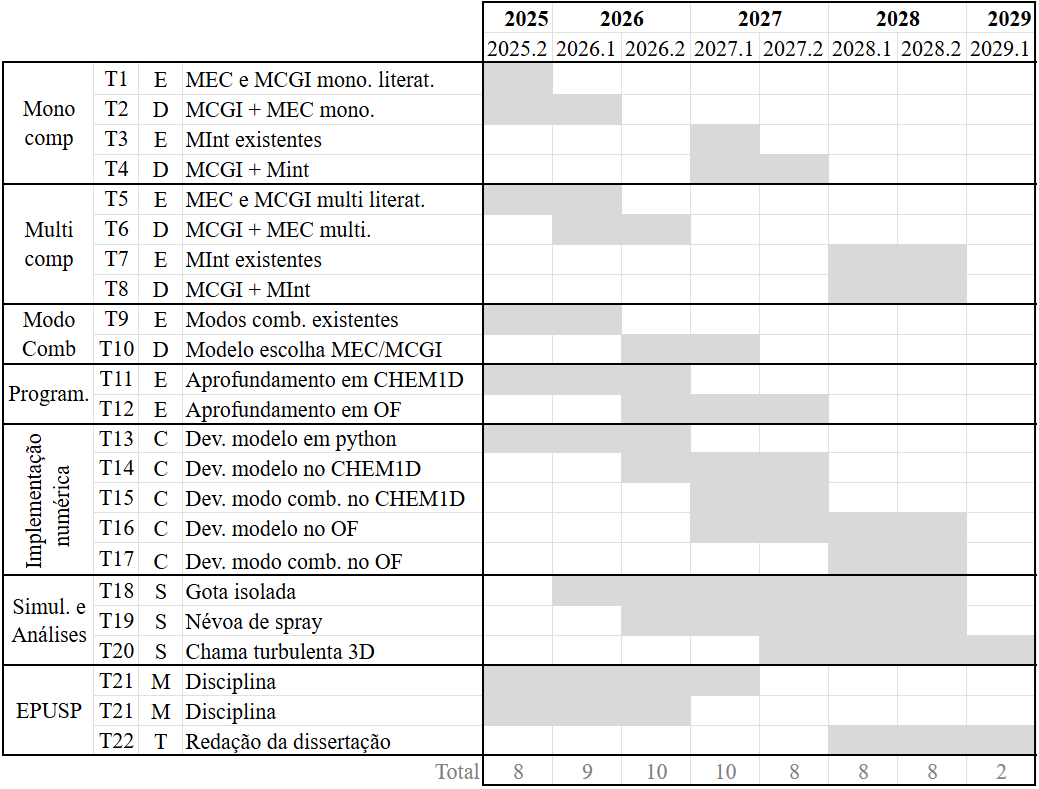
\includegraphics[width=0.85\textwidth]{30_images/cronograma-3.png}
    \label{fig:cronograma}
\end{figure}


O cronograma de execução para as tarefas estabelecidas para esse trabalho pode ser encontrado na Figura \ref{fig:cronograma}.
Considerando inicialmente gotas monocomponentes, o trabalho proposto se iniciará com o estudo aprofundado sobre MEC e MCGI monocomponentes pré-existentes na literatura (tarefa \textbf{T1}), o que dará base para o desenvolvimento de modelo integral de combustão de gota isolada monocomponente com modelo detalhado de evaporação (tarefa \textbf{T2}).
Em sequência virá o estudo aprofundado de modelos preexistentes para a consideração de fenômenos de transporte no interior de gota (tarefa \textbf{T3}), seguido pela avaliação da viabilidade de acoplamento de modelos monocomponente de combustão de gota isolada com modelos para o interior da gota (tarefa \textbf{T4}).
A mesma sequência de tarefas procede para gotas multicomponentes, originando respectivamente as tarefas (\textbf{T5}), (\textbf{T6}), (\textbf{T7}) e (\textbf{T8}). 

Visando utilizar o MCGI desenvolvido em simulações de combustão de spray, faz-se necessário então o estudo aprofundado de modelos de modo de combustão de sprays (\textbf{T9}), focando no modo de combustão de gota isolada e de combustão externa. Em seguida propõe-se o desenvolvimento de um modelo para determinar se a gota utiliza um MEC ou MCGI, baseado nos modelos preexistentes na literatura. (\textbf{T10}).

Para simular os modelos desenvolvidos, é necessário implementá-los no programa a ser utilizado.
Assim, torna-se fundamental o estudo aprofundado dos \emph{softwares} e das linguagens de programação empregadas. 
No caso da simulação em ambiente simplificado, isso envolve o \emph{software} CHEM1D e a linguagem Fortran (\textbf{T11}).
Já para a simulação turbulenta multidimensional, envolve o \emph{software} OpenFOAM e a linguagem C++ (\textbf{T12}).
% Em ambos os casos, o aprofundamento na linguagem de programação visa a implementação do modelo desenvolvido no software utilizado.

Dessa forma, as próximas tarefas abordam a implementação dos MEC e MCGIs desenvolvidos: na linguagem Python  (\textbf{T13}), no  CHEM1D à  (\textbf{T14}) e no OpenFOAM  (\textbf{T16}).
Nos dois últimos, é necessário também implementar o algoritmo de seleção entre MEC e MCGI, originando (\textbf{T15}) e (\textbf{T17}).  
% As tarefas (\textbf{T15}) e (\textbf{T17}) referem-se à implementação do algorítmo do modelo de modo de combustão, que fará a escolha entre MEC e MCGI, nos softwares CHEM1D e OpenFOAM respectivamente.

As primeiras simulações dos modelos desenvolvidos são simulações 0D de evolução temporal de gota isolada em Python (\textbf{T18}). 
Em seguida, vêm as simulações de chama combustão laminar em névoa quiescente de spray no CHEM1D (\textbf{T19}).
Por fim, após aprofundamento em interação chama-turbulência, virão as simulações de chama multidimensional turbulenta no OpenFOAM nas grandes escalas, usando LES, FGM, ATG, e os modelos novos (\textbf{T20}).
As tarefas de simulação detalhadas aqui incluem o pré-processamento, o tempo de simulação e a análise dos resultados (pós-processamento).
As ferramentas utilizadas para a análise dos resultados em cada uma das atividades de simulação são discutidas na Seção \ref{sec:resultados}.

O Programa de Pós-Graduação em Engenharia Mecânica (PPGEM) da EPUSP exige que 9 disciplinas sejam cursadas para doutorado direto.
Elas são representadas pela tarefa (\textbf{T21}).
Algumas disciplinas se destacam devido a sua conexão direta com o tema deste projeto: Fundamentos de Combustão I (PME5228), Fundamentos de Escoamentos Turbulentos Reativos (PME5411), Sistemas Particulados (PQI5848), Termodinâmica Avançada I (PME5014), Introdução à Mecânica dos Meios Contínuos (PME5011) e Modelagem de Turbulência para CFD (PME5418).
Demais disciplinas serão definidas ao longo do desenvolvimento deste trabalho.
Por fim, a redação da dissertação é representada pela tarefa (\textbf{T22}).



% \begin{itemize}
% \setlength{\itemsep}{0cm}
% \item[\textbf{T1}] Estudo aprofundado sobre MEC e MCGI monocomponentes pré-existentes na literatura.% Sobre o MEC, estão incluidos o estudo da derivação dos modelos de Abramzon-Sirignano \cite{Sirignano1989}, a formulação de Miller \cite{MillerR1998}, \todo{...}, No que tange a MCGIs, revisitar o modelo de Godsave-Spalding \cite{Law1978,HenningsJ2024MT}, estudar o artigo do Fachini \cite{FachiniF1999}, suas referências e citações, \todo{...} 
% \item[\textbf{T2}] Modelagem analítica de combustão de gota isolada monocomponente com modelo detalhado de evaporação. % Essa tarefa baseia-se na incorporação do modelo de Abramzon-Sirignano \cite{Sirignano1989} ou da formulação de Miller \cite{MillerR1998} no modelo de Godsave-Spalding \cite{Law1978}. %Como todos os modelos citados baseiam-se em soluções analíticas, é visto como provável que 
% \item[\textbf{T3}] Estudo de modelos preexistentes para a modelagem  analítica de discretização do interior de gota monocomponente.% São exemplos de literatura relevante para essa tarefa \source{}.
% \item[\textbf{T4}] Avaliação da viabilidade de acoplamento de modelos monocomponente de combustão de gota isolada com discretização no interior da gota.% Como os modelos de discretização de interior de gota podem envolver soluções numéricas, se será possível desenvolver uma solução analítica para esse problema. Uma solução acoplada numérica-analítica, interna e externamente gota, respectivamente, precisa ser robusta e computacionalmente eficiente para servir em aplicações CFD. 

% \item[\textbf{T5}] Estudo de modelos MEC e MCGI multicomponente preexistentes na literatura.% Exemplos de trabalhos relevantes de MEC multicomponente incluem \source{}.
% \item[\textbf{T6}] Modelagem analítica de combustão de gota isolada multicomponente com modelo avançado de evaporação. % Essa tarefa baseia-se na incorporação dos modelos de Sacomano \cite{SacomanoF2022IJHMT} ou de Wang \source{WangC2012} no modelo de Godsave-Spalding \cite{Law1978}.
% \item[\textbf{T7}] Estudo de modelos preexistentes para a modelagem analítica de discretização do interior de gota multicomponente.% São exemplos de literatura relevante para essa tarefa \source{}
% \item[\textbf{T8}] Avaliação da viabilidade de acoplamento de modelos multicomponente de combustão de gota isolada com discretização no interior da gota. 

% \item[\textbf{T9}] Estudo de modelos de determinação de modos de combustão de gotas de spray, focando no modo de combustão isolada.% São exemplos de literatura relevante para essa tarefa \cite{AggarwalS2014}, \source{}
% \item[\textbf{T10}] Desenvolvimento de modelo analítico para escolha entre MEC e MCGI, baseado na pesquisa do item anterior.

% \item[\textbf{T11}] Aprofundamento em CHEM1D e em Fortran para programação no CHEM1D.
% \item[\textbf{T12}] Aprofundamento em OpenFOAM e em C++ para programação no OpenFOAM.

% \item[\textbf{T13}] Implementação do modelo MEC/MCGI em Python.% para o T18.
% \item[\textbf{T14}] Implementação do modelo MEC/MCGI no CHEM1D.% para o T19.
% \item[\textbf{T15}] Implementação do modelo de modo de combustão no CHEM1D.
% \item[\textbf{T16}] Implementação do modelo MEC/MCGI no OpenFOAM.% para o T20.
% \item[\textbf{T17}] Implementação do modelo de modo de combustão no OF.

% \item[\textbf{T18}] Simulação da evolução temporal 0D de gota isolada em Python.           %, após T15.
% \item[\textbf{T19}] Simulação de combustão laminar de névoa quiescente de spray no CHEM1D. %, após T16.
% \item[\textbf{T20}] Simulação de chama turbulenta 3D nas grandes escalas com FGM e ATF.    %, após T17.

% \item[\textbf{T21}] Disciplinas de pós-graduação.% No programa de Doutorado Direto do PPGEM na POLI-USP, é necessário cursar 9 Disciplinas, cada valendo 8 créditos. Como não é recomendado cursar mais de duas disciplinas por oferencimento, o qual é quadrimestral, as disciplinas serão cursadas ao longo de 5 quadrimestres, aproximadamente 2 anos. Algumas das disciplinas a serem cursadas já foram escolhidas e estão dispostas na Seção \ref{sec:disciplinas}.
% \item[\textbf{T22}] Redação da dissertação.% Estimou-se iniciar a escrita da dissertação nos últimos três semestres.
% \end{itemize}

         % Plano de Trabalho e Cronograma de Excecução
% !TEX root = ../Proposta.tex

\section{Forma de Análise dos Resultados} \label{sec:resultados}

Diferentes procedimentos serão adotados para a análise dos resultados obtidos em cada etapa de trabalho apresentada na Seção \ref{sec:metod}.
Considerando apenas os resultados numéricos, i.e. das de simulações, os primeiros resultados serão obtidos após o teste do modelo isolado.

A simulação da evolução temporal de um modelo de gota, MEC ou MCGI, e a análise desses resultados é uma área que o autor da proposta já tem experiência \cite{HenningsJ2024MT}. 
Nessa análise, são relevantes parâmetros como o tempo de vida da gota, a dependência dos resultados de condições iniciais da gota e do ambiente e a dependência dos submodelos utilizados, como o de pressão de vapor ou de fração molar de vapor.

No contexto de avaliação isolada de MECs e MCGIs, é de extrema relevância a comparação com resultados tanto experimentais e quanto de estudos numéricos detalhados.
Para MECs, consideram-se, por exemplo, os trabalhos experimentais \cite{BiroukM2006,PatelU2019,KayaEyiceD2024,ArabkhalajA2024,MaquaC2008}, focados na influência da turbulência na evaporação.
Para MCGIs, consideram-se os trabalhos experimentais na escala da gota \cite{ChoS1990SCI,CandelS1999,ChenG1996CF,Xu2002,BiroukM2000,CuociA2005,SetyawanH2015} e os trabalhos baseados em DNS que resolvem o modelo da gota \cite{Stauch2006,CuociA2005,ChoS1990SCI,KazakovA2003CF,MarcheseA1996CF,WangW2024}.

Já para as simulações em ambiente simplificado, a análise dos resultados se dará baseada na experiência do grupo de pesquisa, assim como na comparação com MECs já desenvolvidos pelo grupo e testados nesse ambiente \cite{SacomanoF2018CTM,SacomanoF2019IJHMT,SacomanoF2021Fluids,SacomanoF2024CF,SacomanoF2025CF}.
Nessas simulações, são relevantes a influência das condições iniciais e ambientais na frente de chama, em particular na velocidade de chama laminar.
Esse ambiente é muito importante para análises paramétricas e preliminares.

Nas simulações multidimensionais, também será valiosa a experiência e os resultados anteriores do grupo de pesquisa \cite{SacomanoF2017CF,SacomanoF2020CF}.
Elas possibilitarão estudar a influência do modo de combustão de gota isolada na estrutura da chama, como proposto nos objetivos do trabalho.    % Resultados Esperados // Forma de análise dos resultados


\newpage
\newpage
\pagenumbering{roman}
\setcounter{page}{\value{savecounter}}

% \bibliographystyle{abntex2-alf}
\bibliographystyle{unsrt}
\bibliography{bibliography,bibliography2}


\end{document}
